\section{Web App}

\subsection{Requisiti}
Per poter utilizzare correttamente la web app è necessario disporre di una connessione ad internet e di un browser web che supporti l'estensione Metamask. L'applicazione è stata testata sui seguenti browser:
\begin{itemize}
    \item Google Chrome v112;
    \item Mozilla Firefox v112;
    \item Microsoft Edge v112.
\end{itemize}
L'unico tra i principali browser che non supporta Metamask è Safari, pertanto non è possibile utilizzare la web app su tale browser.

\subsubsection{MetaMask}
Per poter utilizzare la web app è necessaria un'installazione funzionante dell'estensione MetaMask per il browser web.

MetaMask è un portafoglio digitales che permette di interagire con la blockchain Ethereum e con gli smart contract eseguiti su di essa, offrendo la possibilità di effettuare transazioni con diverse criptovalute.

Per le istruzioni di installazione e configurazione di MetaMask si rimanda alla \href{https://support.metamask.io/hc/en-us/articles/360015489531-Getting-started-with-MetaMask}{documentazione ufficiale}.

\subsection{Funzionalità}
All'apertura della web app, verrà visualizzata la pagina principale. La maggior parte delle funzionalità sarà disponibile solo dopo aver effettuato l'accesso con MetaMask; i bottoni corrispondenti a tali features saranno disabilitati fino ad allora.

\begin{figure}[H]
    \minipage{0.45\textwidth}
      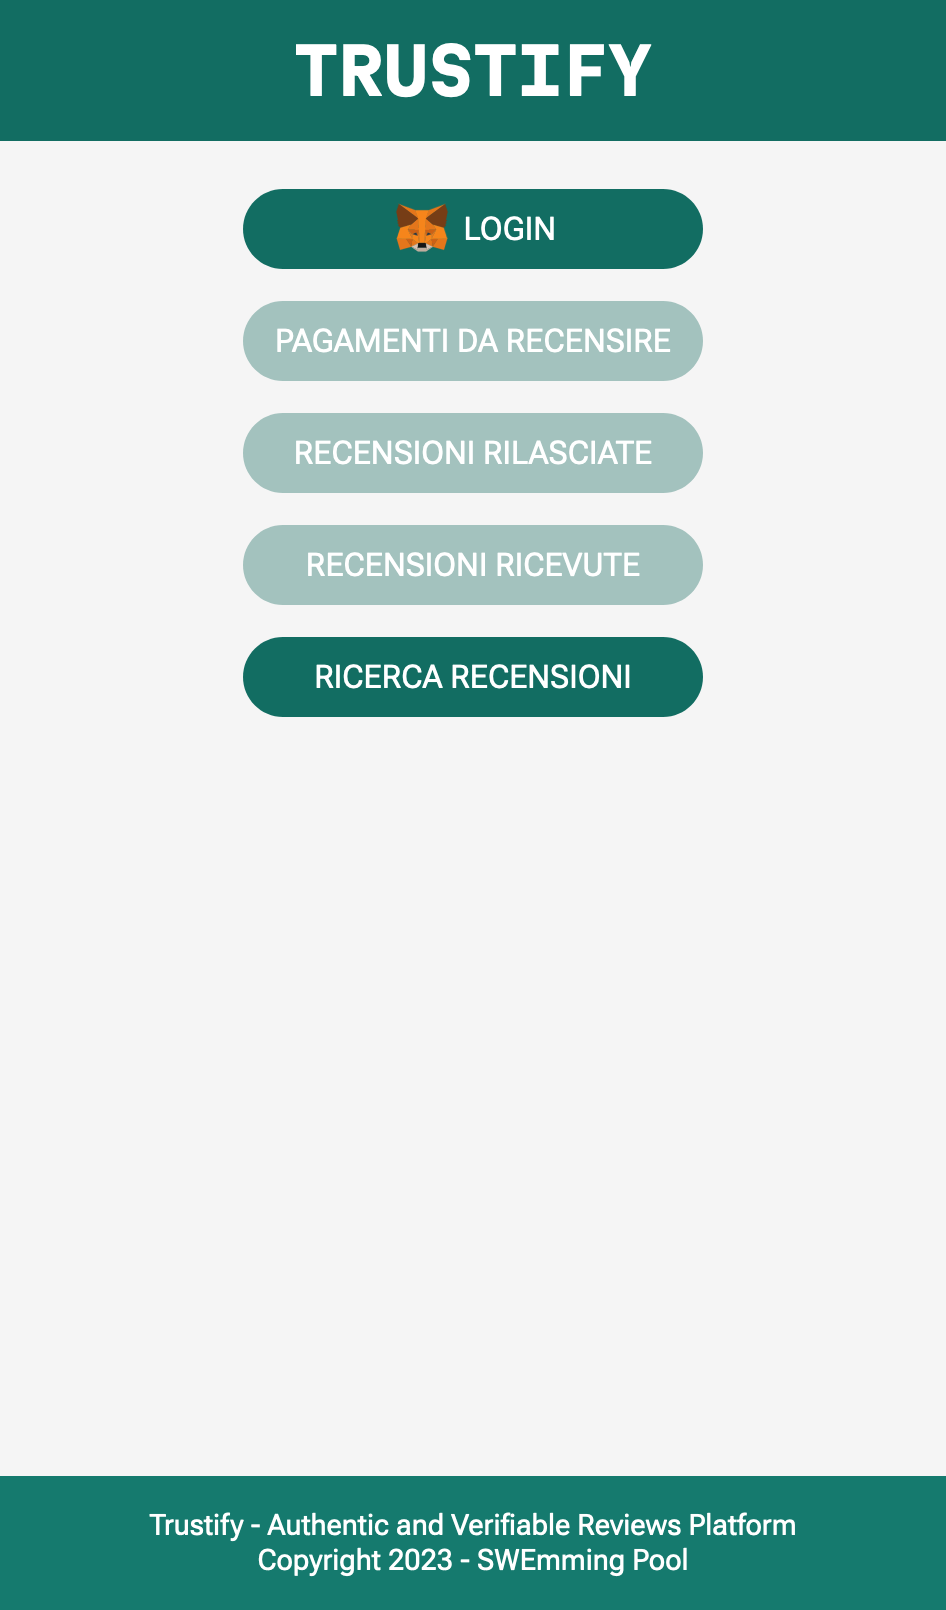
\includegraphics[width=\linewidth]{src/img/home.png}
      \caption{Pagina Home}\label{fig:home}
    \endminipage\hfill
    \minipage{0.45\textwidth}
      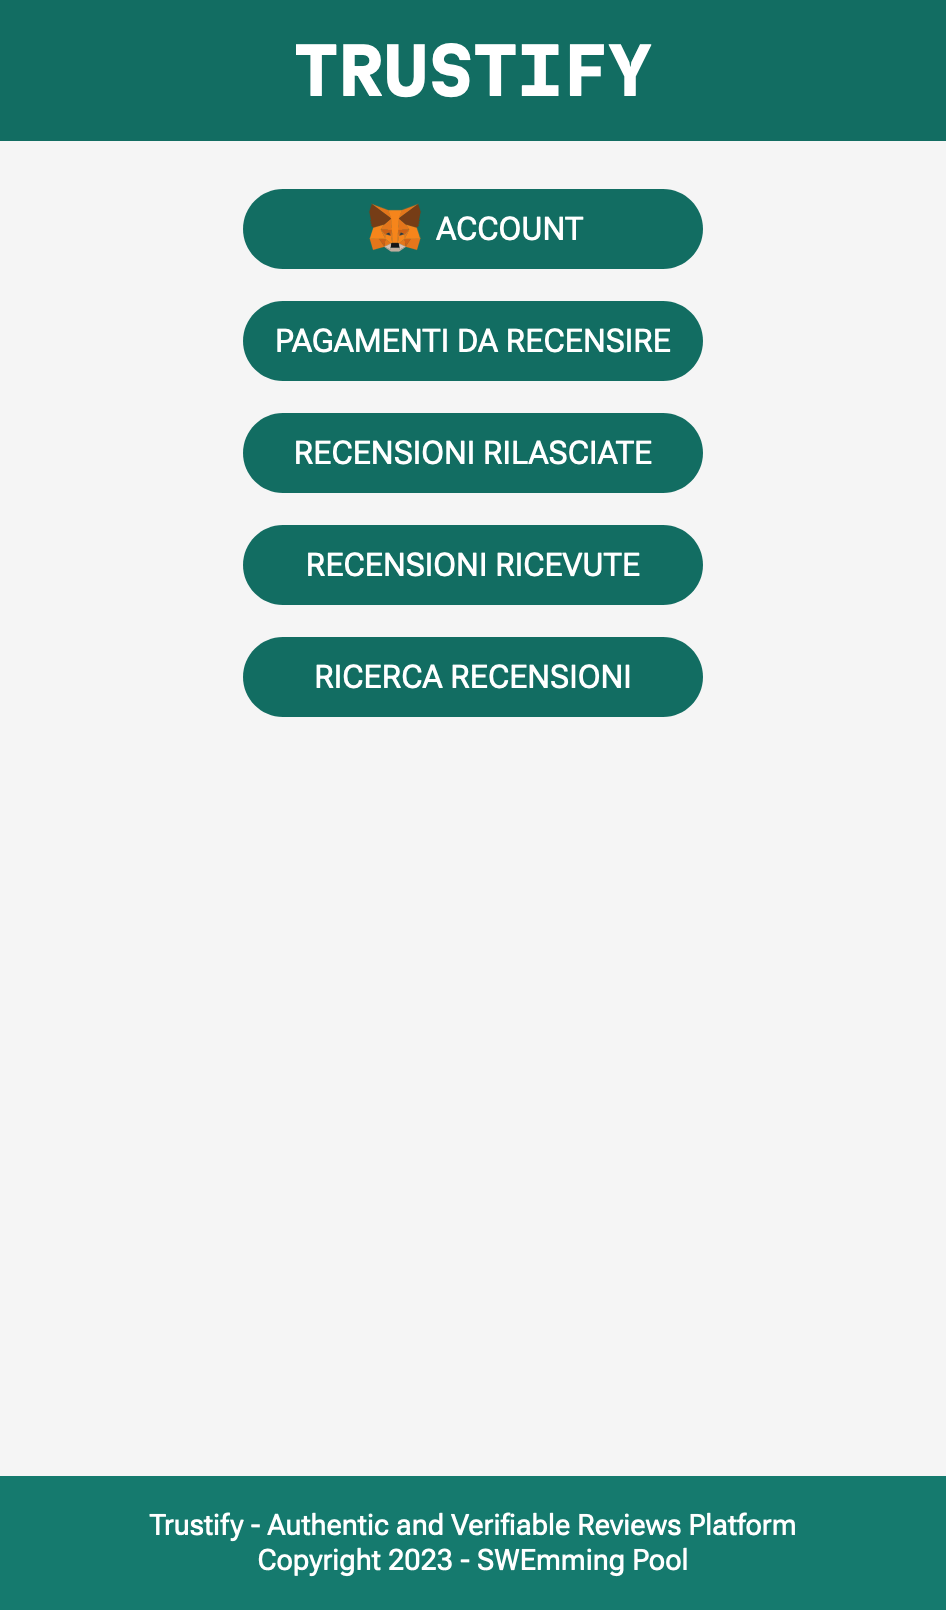
\includegraphics[width=\linewidth]{src/img/home_login.png}
      \caption{Pagina Home a login effettuato}\label{fig:home_login}
    \endminipage\hfill
\end{figure}

Non è presente un bottone per effettuare pagamenti, in quanto il checkout, nella versione finale, sarà integrato direttamente nel sito web del commerciante, e dati quali indirizzo e prezzo da pagare non saranno modificabili dall'utente. È comunque possibile testare la funzionalità di pagamento come spiegato di seguito.

\subsubsection{Checkout}
Per motivi di test, è stato implementato un checkout di prova, accessibile inserendo nell'URL indirizzo del destinatario e quantità di ETH da inviare. Se, per esempio, la web app fosse hostata su \path{https://trustify.com}, l'URL avrebbe la seguente forma: \path{https://trustify.com/checkout/indirizzo-wallet/quantita-eth}.

Cliccando sul bottone "Paga con Trustify", verrà aperta una finestra di Metamask per confermare la transazione, e si sarà reindirizzati all'interno della web app. Una volta confermata, verrà visualizzata una pagina di conferma del pagamento.

\begin{figure}[H]
    \minipage{0.32\textwidth}
      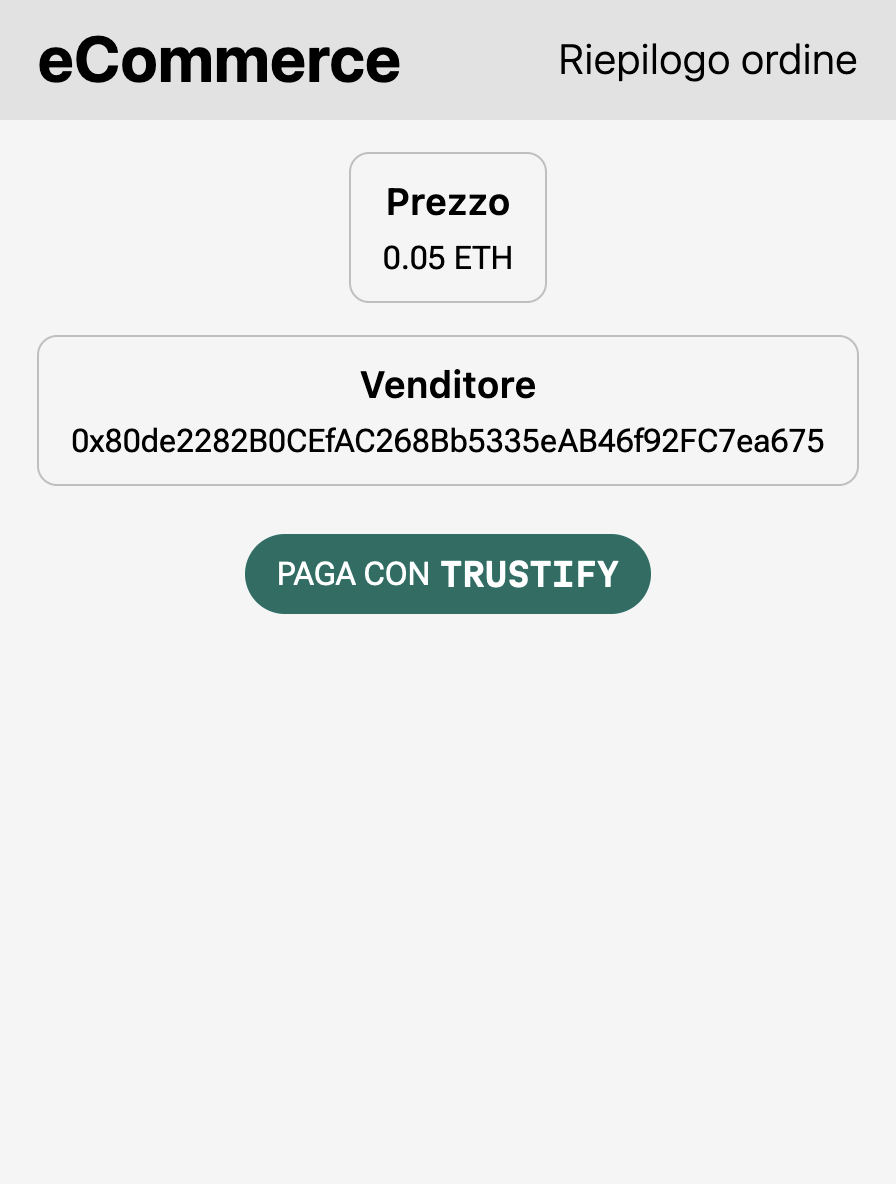
\includegraphics[width=\linewidth]{src/img/checkout.png}
      \caption{Pagina di checkout fittizia}\label{fig:checkout}
    \endminipage\hfill
    \minipage{0.32\textwidth}
      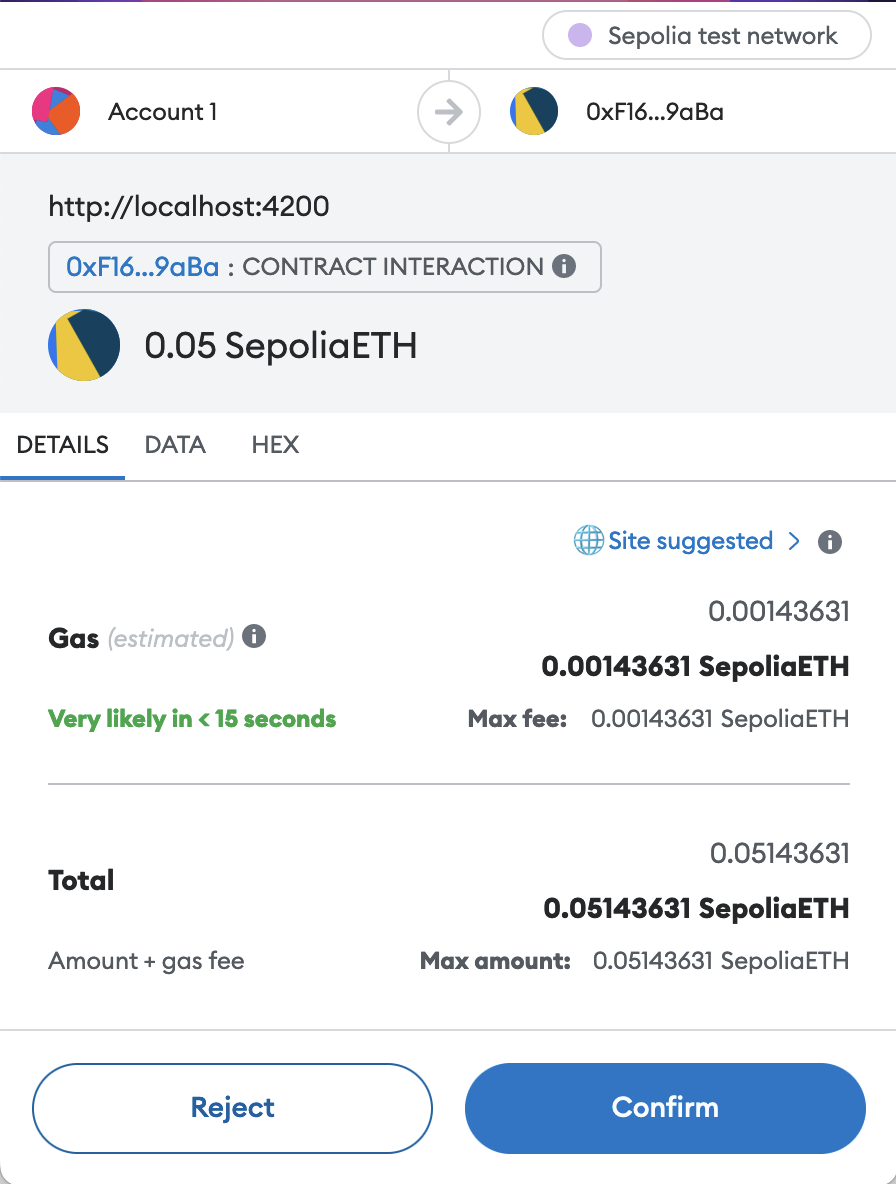
\includegraphics[width=\linewidth]{src/img/checkout_metamask.png}
      \caption{Popup di pagamento su MetaMask}\label{fig:checkout_metamask}
    \endminipage\hfill
    \minipage{0.32\textwidth}%
      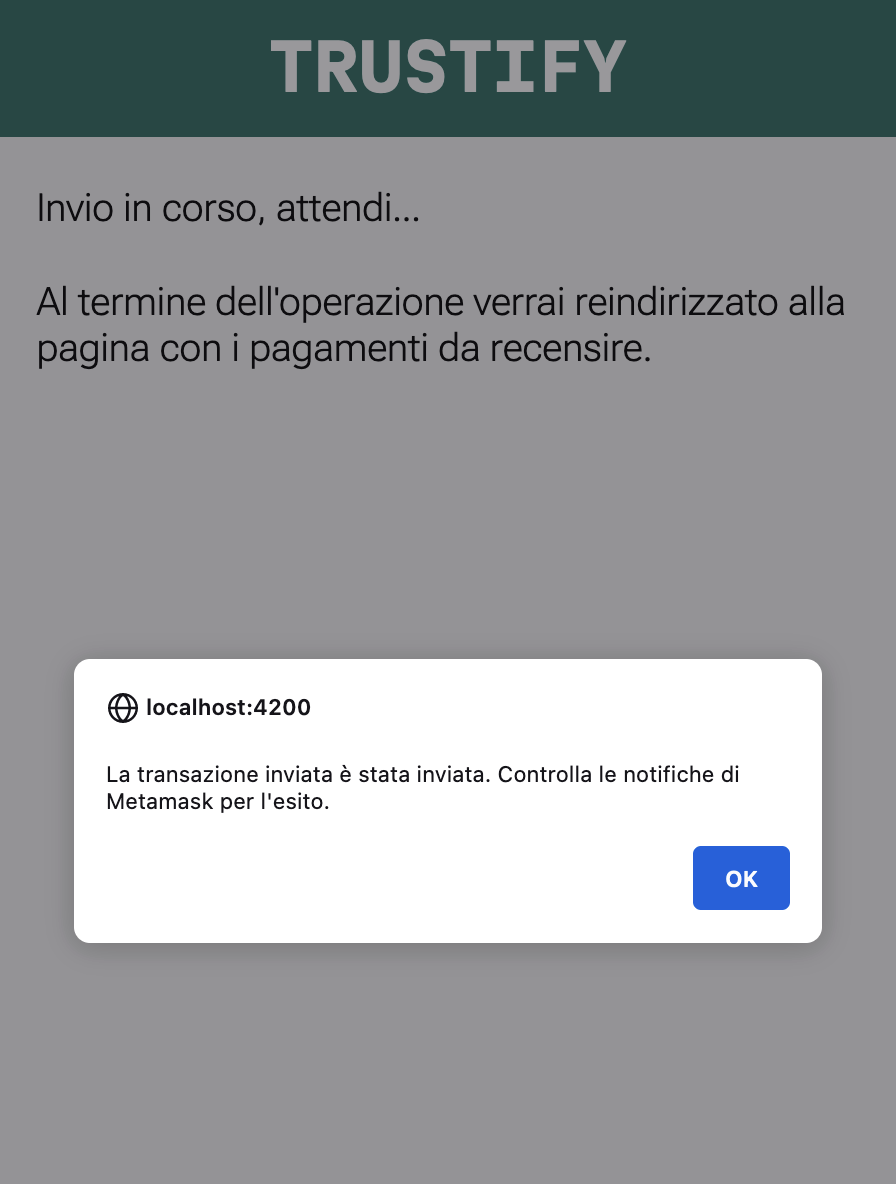
\includegraphics[width=\linewidth]{src/img/checkout_conferma.png}
      \caption{Pagina di attesa e conferma pagamento}\label{fig:checkout_conferma}
    \endminipage
\end{figure}

\subsubsection{Login/Account}
Per effettuare il login, è necessario cliccare sul bottone "Login" e confermare l'accesso su MetaMask. Una volta effettuato il login, il bottone cambierà nome in "Account" e permetterà di visualizzare l'indirizzo del wallet utilizzato per l'accesso.

\begin{figure}[H]
    \minipage{0.32\textwidth}
      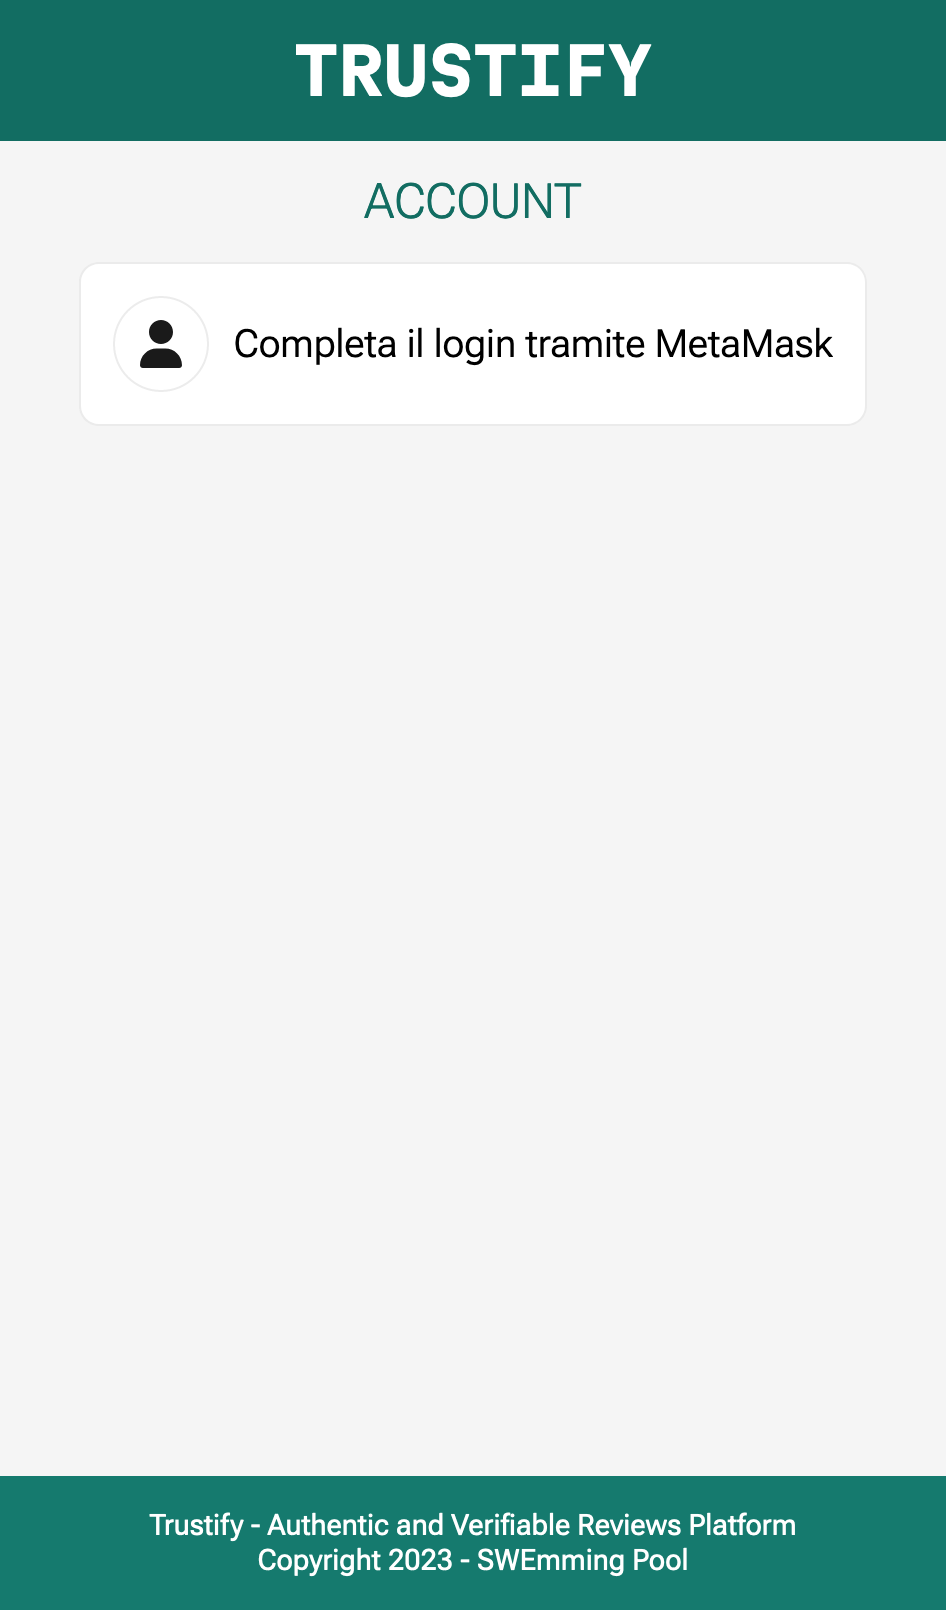
\includegraphics[width=\linewidth]{src/img/login.png}
      \caption{Pagina di login}\label{fig:login}
    \endminipage\hfill
    \minipage{0.32\textwidth}
      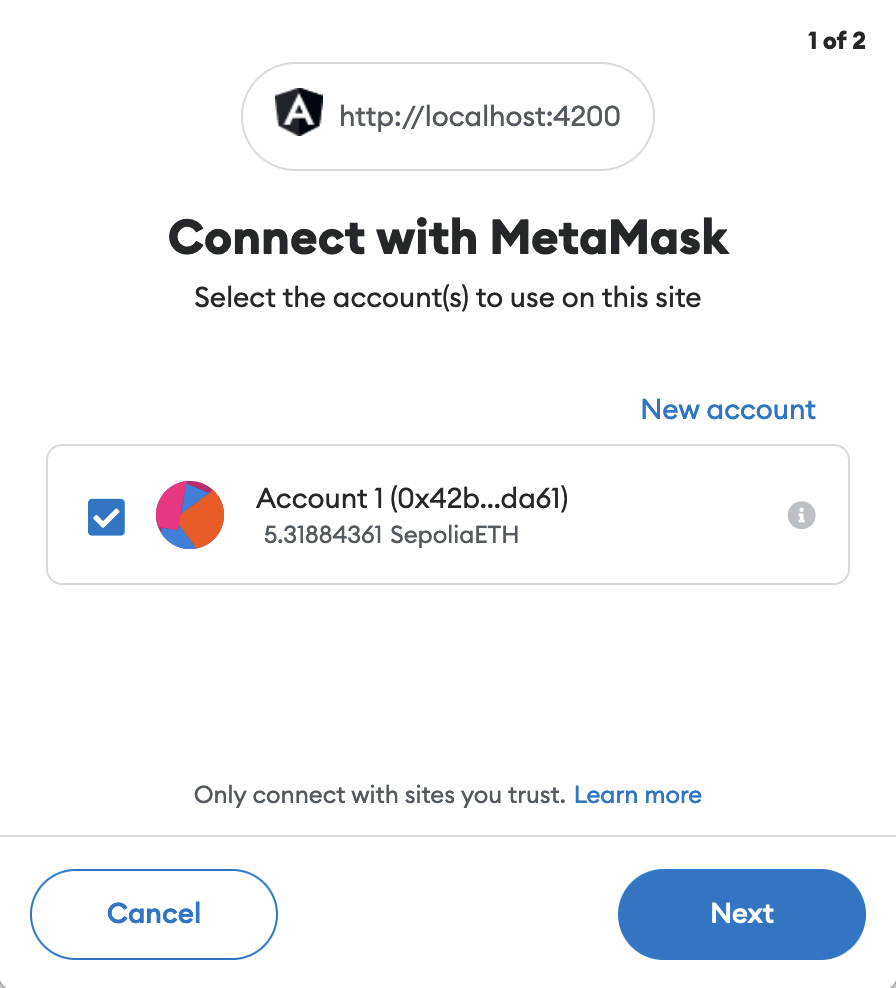
\includegraphics[width=\linewidth]{src/img/login_metamask.png}
      \caption{Popup di login su MetaMask}\label{fig:login_metamask}
    \endminipage\hfill
    \minipage{0.32\textwidth}%
      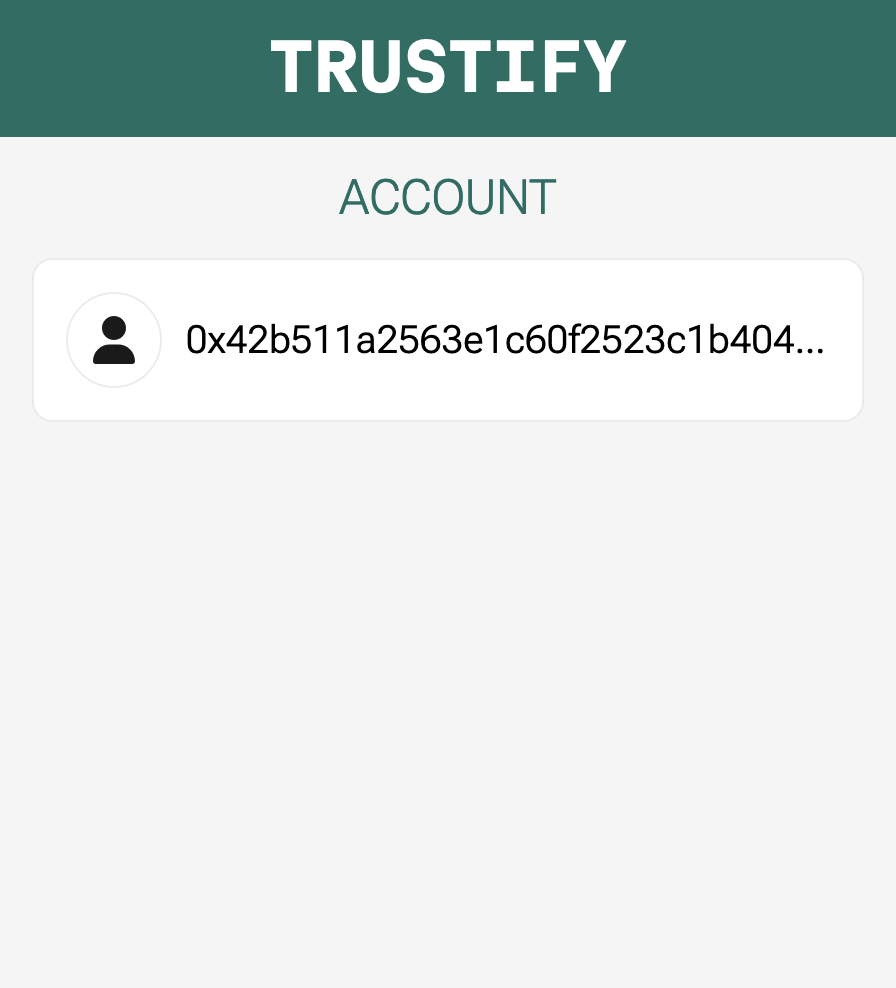
\includegraphics[width=\linewidth]{src/img/account.png}
      \caption{Pagina con l'indirizzo del proprio wallet}\label{fig:account}
    \endminipage
\end{figure}


\subsubsection{Pagamenti da recensire}

\subsubsection{Recensioni rilasciate}

\subsubsection{Recensioni ricevute}

\subsubsection{Ricerca recensioni}